\documentclass[12pt]{article}

\usepackage{amsmath}
\usepackage{unicode-math}
\usepackage{xltxtra}
\usepackage{xgreek}

\setmainfont{Liberation Serif}

\usepackage{tabularx}

\pagestyle{empty}

\usepackage{geometry}
 \geometry{a4paper, total={190mm,280mm}, left=10mm, top=10mm}

 \usepackage{graphicx}
 \graphicspath{ {images/} }

 \usepackage{wrapfig}
\usepackage{lipsum}%% a garbage package you don't need except to create examples.

\begin{document}

\begin{table}
    \small
    \begin{tabularx}{\textwidth}{ c X r }
      \begin{tabular}{ c }
        
\includegraphics[scale=0.4]{logo} \\
        ΕΛΛΗΝΙΚΗ ΔΗΜΟΚΡΑΤΙΑ \\
        ΥΠΟΥΡΓΕΙΟ ΠΑΙΔΕΙΑΣ, ΕΡΕΥΝΑΣ \& ΘΡΗΣΚΕΥΜΑΤΩΝ \\
        ΠΕΡΙΦΕΡΕΙΑΚΗ Δ/ΝΣΗ ΠΡΩΤ. \& ΔΕΥΤ/ΜΙΑΣ  ΕΚΠ/ΣΗΣ \\
        ΚΕΝΤΡΙΚΗΣ ΜΑΚΕΔΟΝΙΑΣ \\
        Δ/ΝΣΗ ΔΕΥΤΕΡΟΒΑΘΜΙΑΣ ΕΚΠ/ΣΗΣ ΑΝ. ΘΕΣ/ΝΙΚΗΣ \\
        27ο ΓΕΝΙΚΟ ΛΥΚΕΙΟ ΘΕΣ/ΝΙΚΗΣ
      \end{tabular}
      & &
      \begin{tabular}{ r }
        Σχολικό Έτος: 2016 - 2017 \\
        Εξ. Περίοδος: Μαΐου - Ιουνίου \\
        Μάθημα: Γεωμετρία Α Λυκείου\\
        Εισηγητές: Λόλας, Τερζόγλου, Χ''Σάββας \\ \\
        Θεσσαλονίκη, 22 / 05 / 2017
      \end{tabular}
    \end{tabularx}
\end{table}

\part*{\centering{Θέματα}}

\section*{Θέμα Α}
  \noindent
  \begin{enumerate}
    \item \textbf{[Μονάδες 15]} Να αποδείξετε ότι το άθροισμα των γωνιών κάθε τριγώνου είναι $2$ ορθές.
    \item \textbf{[Μονάδες 10]}  Να χαρακτηρίσετε τις παρακάτω προτάσεις με Σωστό ή Λάθος
    \begin{enumerate}
      \item [α)] Παραλληλόγραμμο λέγεται το τετράπλευρο που έχει τις απέναντι πλευρές του παράλληλες.
      \item [β)] Οι διαγώνιοι του ρόμβου τέμνονται κάθετα.
      \item [γ)] Σε κάθε ορθογώνιο τρίγωνο η διάμεσος που αντιστοιχεί στην υποτείνουσα είναι ίση με το μισό αυτής.
      \item [δ)] Αν δύο γωνίες έχουν τις πλευρές τους κάθετες μία προς μία, είναι πάντα ίσες.
      \item [ε)] Δύο χορδές ενός κύκλου είναι ίσες αν και μόνο αν τα αποστήματά τους είναι ίσα.
    \end{enumerate}
  \end{enumerate}

\section*{Θέμα Β}
  \noindent
  \begin{wrapfigure}[4]{r}{0.3\textwidth}
    \centering
    \vspace{-60pt}
    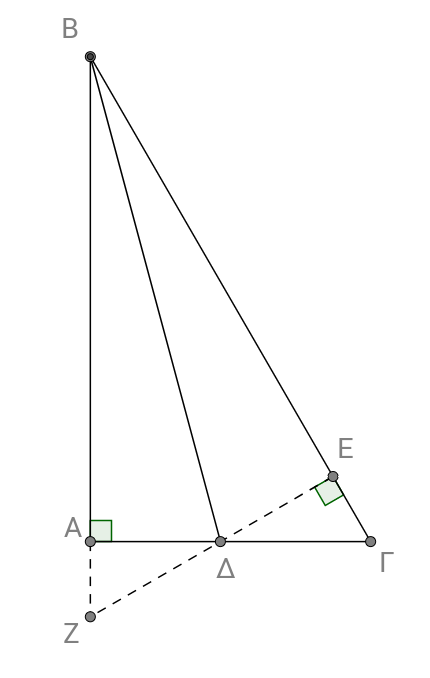
\includegraphics[width=0.3\textwidth]{2017AGeo2}
  \end{wrapfigure}
  Δίνεται ορθογώνιο τρίγωνο $\overset{\triangle}{ΑΒΓ}$, $\left( \hat{Α}= 90^{\circ} \right)$ και η διχοτόμος του $ΒΔ$. Από το $Δ$ φέρνουμε $ΔΕ \bot ΒΓ$, που τέμνει την $ΑΒ$ στο $Ζ$. Να αποδείξετε ότι:
  \begin{enumerate}
    \item \textbf{[Μονάδες 10]} $ΔΑ=ΔΕ$.
    \item \textbf{[Μονάδες 15]} Το τρίγωνο $\overset{\triangle}{ΒΓΖ}$ είναι ισοσκελές.
  \end{enumerate}
  %\vspace{7\baselineskip}
  \newpage

\section*{Θέμα Γ}
  \noindent
  \begin{wrapfigure}[4]{r}{0.4\textwidth}
    \centering
    \vspace{-50pt}
    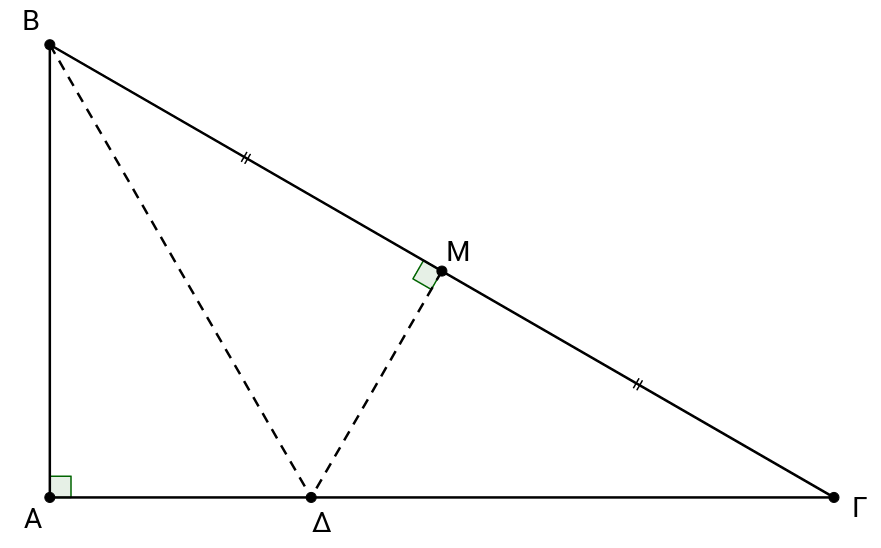
\includegraphics[width=0.4\textwidth]{2017AGeo3}
  \end{wrapfigure}
  Σε ορθογώνιο τρίγωνο $\overset{\triangle}{ΑΒΓ}$, $\left( \hat{Α}=  90^{\circ} \right)$ με $\hat{Γ}=30^{\circ}$, η μεσοκάθετη της υποτείνουσας $ΒΓ$ τέμνει την πλευρά $ΑΓ$ στο $Δ$. Να αποδείξετε ότι:
  \begin{enumerate}
    \item \textbf{[Μονάδες 12]} Το ευθύγραμμο τμήμα $ΒΔ$ είναι διχοτόμος της γωνίας $\hat{Β}$.
    \item \textbf{[Μονάδες 13]} $ΔΜ=\frac{ΑΓ}{3}$
  \end{enumerate}

\section*{Θέμα Δ}
  \noindent
  \begin{wrapfigure}[4]{r}{0.4\textwidth}
    \centering
    \vspace{-50pt}
    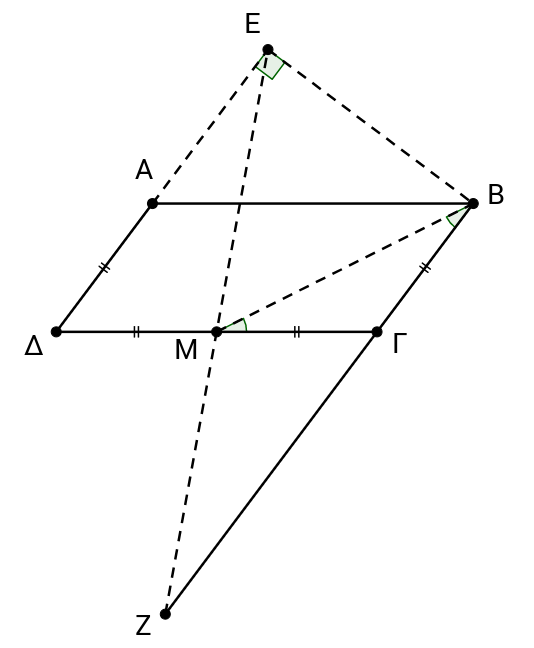
\includegraphics[width=0.4\textwidth]{2017AGeo4}
  \end{wrapfigure}
  Στο παραλληλόγραμμο $ΑΒΓΔ$ η $ΑΒ=2ΒΓ$ η γωνία $\hat{Α}>90^{\circ}$, $Μ$ μέσο της $ΔΓ$, η $ΒΕ$ κάθετη στην προέκταση της $ΔΑ$ και η $ΕΜ$ τέμνει την προέκταση της $ΒΓ$ στο $Ζ$.
  \begin{enumerate}
    \item \textbf{[Μονάδες 6]}  Να αποδείξετε ότι $\widehat{ΓΒΜ}=\widehat{ΓΜΒ}$
    \item \textbf{[Μονάδες 9]}  Να δείξετε ότι τα τρίγωνα $ΔΕΜ$ και $ΜΓΖ$ είναι ίσα.
    \item \textbf{[Μονάδες 3]}  Να δείξετε ότι το τρίγωνο $\overset{\triangle}{ΕΒΖ}$ είναι ορθογώνιο στην γωνία $\widehat{ΕΒΖ}$.
    \item \textbf{[Μονάδες 7]}  Να δείξετε ότι $ΜΒ=ΜΖ$
  \end{enumerate}

\vspace{3\baselineskip}

\part*{\centering{Καλή επιτυχία}}
\begin{table}[htb]
    \begin{tabularx}{\textwidth}{ X c X c X}
      &
      \begin{tabular}[t]{ c }
        Ο Δ/ντης
        \\ \\ \\ \\ \\
        Δρ. Ιωαννίδης Νικόλαος
      \end{tabular}
      & &
      \begin{tabular}[t]{ c }
        Οι εισηγητές \\ \\
        \multicolumn{1}{l}{1. Λόλας Κωνσταντίνος} \\ \\
        \multicolumn{1}{l}{2. Τερζόγλου Ιωάννης} \\ \\
        \multicolumn{1}{l}{3. Χ''Σάββας Δημήτριος}
      \end{tabular}
      &
    \end{tabularx}
\end{table}

\vspace*{\fill}
 \textbf{Οδηγίες}
 \begin{enumerate}
   \item Να απαντήσετε σε όλα τα θέματα
   \item Μην ξεχάσετε να γράψετε το ονοματεπώνυμό σας σε κάθε φύλλο απαντήσεων που σας δώσουν.
   \item Όλες οι απαντήσεις να δωθούν στο φύλλο απαντήσεων. Οτιδήποτε γραφτεί στη σελίδα με τα θέματα δεν θα ληφθεί υπόψιν.
   \item Τα Σωστό - Λάθος δεν χρειάζονται αιτιολόγηση.
 \end{enumerate}
\end{document}
